\documentclass[border=4pt]{standalone}
% Preámbulo común de las figuras. Cada figura es un documento standalone
% que se compila a SVG con scripts/build_figures.sh
\usepackage[utf8]{inputenc}
\usepackage{amsmath}
\usepackage{tikz}
\usepackage[american, siunitx]{circuitikz}
\usetikzlibrary{arrows.meta,calc,decorations.pathmorphing,patterns}
\tikzset{
  >={Stealth[length=2.2mm]},
  eje/.style={->, thin},
  hilo/.style={thick},
}
% Paleta común: tonos medios legibles sobre fondo claro
\definecolor{azul}{RGB}{31,94,168}
\definecolor{rojo}{RGB}{192,57,43}
\definecolor{verde}{RGB}{39,128,73}
\definecolor{naranja}{RGB}{211,120,30}
\definecolor{morado}{RGB}{125,60,152}

\begin{document}
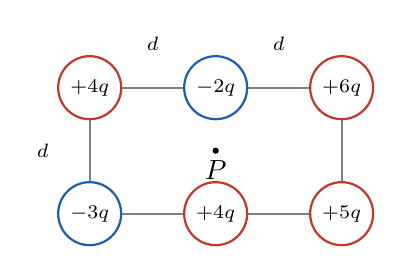
\begin{tikzpicture}[scale=1.0]
  \def\d{1.6}
  \draw[thick, gray] (-\d,-\d/2) rectangle (\d,\d/2);
  \foreach \x/\y/\l/\c in {-1/1/{+4q}/rojo, 0/1/{-2q}/azul, 1/1/{+6q}/rojo, -1/-1/{-3q}/azul, 0/-1/{+4q}/rojo, 1/-1/{+5q}/rojo}
    \node[circle, draw=\c, thick, fill=white, minimum size=0.8cm, inner sep=0pt, font=\scriptsize] at (\x*\d,\y*\d/2) {$\l$};
  \foreach \x in {-0.8,0.8} \node[above=0.35cm, font=\scriptsize] at (\x,\d/2) {$d$};
  \node[left=0.4cm, font=\scriptsize] at (-\d,0) {$d$};
  \fill (0,0) circle (0.04) node[below]{$P$};
\end{tikzpicture}
\end{document}
